\documentclass[11pt]{article}
\usepackage[margin=1in]{geometry}
\usepackage{xcolor}
\usepackage{mdframed}
\usepackage{amsmath}
\usepackage{graphicx}
\usepackage{float}
\usepackage{listings}
\usepackage{booktabs}
\usepackage{hyperref}

\lstset{
    language=Matlab,
    basicstyle=\ttfamily\footnotesize,
    keywordstyle=\color{blue},
    breaklines=true
}

\newcommand{\yourname}{Alex Shaffer, Istiaque Ahmed}
\newcommand{\yournetid}{aws9, miahmed2}
\newcommand{\hwnum}{6}
\newcommand{\probnum}{1}

\newenvironment{problem}[2][Problem]
    { \begin{mdframed}[backgroundcolor=gray!20] \textbf{#1 #2} \\}
    {  \end{mdframed}}

\newenvironment{solution}
    {\textit{Solution:}}
    {}

\begin{document}
\noindent
\noindent\rule{\linewidth}{2pt}
\large\textbf{\yourname} \hfill \textbf{CS 555: Homework \# \hwnum}   \\
Email: \yournetid@illinois.edu \hfill Spring 2026\\
GitHub Repo: \texttt{\url{https://github.com/redhorn144/CS555/}} \\
\noindent\rule{\linewidth}{2pt}

% -------------------------------------------------------
\begin{problem}{1(a)}
\end{problem}

\begin{solution}
For Part 1a, the pressure distribution for the 2D incompressible taper-flat slider bearing was computed using the Finite Element Method. 
The load $F$ and the center-of-pressure $x_p$ were calculated using the following integrals over the domain $\Omega$:
\begin{align*}
    F &= \int_{\Omega} p(x,y) \, dx \, dy \\
    x_p &= \frac{1}{F} \int_{\Omega} x \, p(x,y) \, dx \, dy
\end{align*}

Using the numerical solution, the computed values are:
\begin{itemize}
    \item \textbf{Computed Load ($F$):} $0.2066599$ N
    \item \textbf{Center of Pressure ($x_p$):} $0.002208667$ m
\end{itemize}

\subsection*{Analytical Verification}
The analytical load $\tilde{F}$ for a 1D pure wedge configuration is given by:
\begin{equation*}
    \tilde{F} = \frac{\Lambda L W}{(1-\alpha)^2} \left( \ln(\alpha) + 2 \frac{1-\alpha}{1+\alpha} \right)
\end{equation*}
where $\alpha = h_1/h_2$ and $\Lambda = 6\mu U L / h_2^2$. Substituting the given parameters, we obtain:

\begin{itemize}
    \item \textbf{Analytical Load ($\tilde{F}$):} $8.154767$ N
\end{itemize}

\vspace{0.5cm}

We may compare this to the numerical load $F$ computed from the 2D simulation with the configuration described in part 1b.
This involves setting $Ta = 0$ and using Neumann boundary conditions. We get a numerical load:

\begin{itemize}
    \item \textbf{Numerical Load ($F$):} $8.154072$ N
    \item \textbf{Relative Error: $0.01\%$}
\end{itemize}

\subsection*{Pressure Distribution}
The numerical pressure distribution $p(x,y)$ over the slider domain is shown in Figure \ref{fig:pressure}.

\begin{figure}[ht!]
    \centering
    
\includegraphics[width=0.8\textwidth]{part_1a}
    \caption{Normalized pressure distribution for the incompressible taper-flat slider bearing.}
    \label{fig:pressure}
\end{figure}

\end{solution}

% -------------------------------------------------------
\begin{problem}{1(b)}

\end{problem}

\begin{solution}
To verify the finite element solver against the analytical solution for a 1D wedge bearing, the physical parameters were adjusted to represent a pure wedge. Specifically, the leading taper angle was set to zero ($T_a = 0$), and Neumann boundary conditions were enforced on the top and bottom edges of the domain. This was achieved by applying Dirichlet boundary conditions ($p=0$) exclusively to the leading ($x=0$) and trailing ($x=L$) edges, thus forcing a strictly 1D flow in the $x$-direction.

The analytical solution for the 1D wedge bearing is given by:
\begin{equation}
    \tilde{p}(x) = \frac{\alpha\Lambda}{1-\alpha^2}\left(\frac{1}{H^2} - \frac{1}{\alpha^2}\right) - \frac{\Lambda}{1-\alpha}\left(\frac{1}{H} - \frac{1}{\alpha}\right)
\end{equation}
where $\alpha = h_1/h_2$, $H(x) = \alpha + (1-\alpha)(x/L)$, and $\Lambda = 6\mu UL/h_2^2$.

\subsection*{Convergence Study Results}
A mesh refinement study was performed by varying the number of elements in the $x$-direction ($E_x \in \{15, 30, 60, 120\}$) while keeping $E_y = 40$ constant. The maximum pointwise error between the numerical solution $p(x)$ and the analytical solution $\tilde{p}(x)$ was computed for each mesh resolution.

\begin{table}[H]
    \centering
    \begin{tabular}{|c|c|}
        \hline
        \textbf{Number of Elements ($E_x$)} & \textbf{Max Pointwise Error (Pa)} \\
        \hline
        15  & 2932.079 \\
        30  & 757.7912 \\
        60  & 201.5704 \\
        120 & 56.73146 \\
        \hline
    \end{tabular}
    \caption{Maximum pointwise error in $p(x)$ for different mesh resolutions.}
    \label{tab:convergence_data}
\end{table}

The estimated convergence rate, calculated from the slope of the log-log plot of the error versus $E_x$, is approximately \textbf{$-1.90$}. This value is close to $-2.0$, successfully demonstrating the expected second-order convergence of the linear triangular elements for this problem.

\subsection*{Figures}
Figure \ref{fig:pressure_1d} shows the pressure distribution, while Figure \ref{fig:convergence} illustrates the convergence behavior of the finite element solver.

\begin{figure}[H]
    \centering
    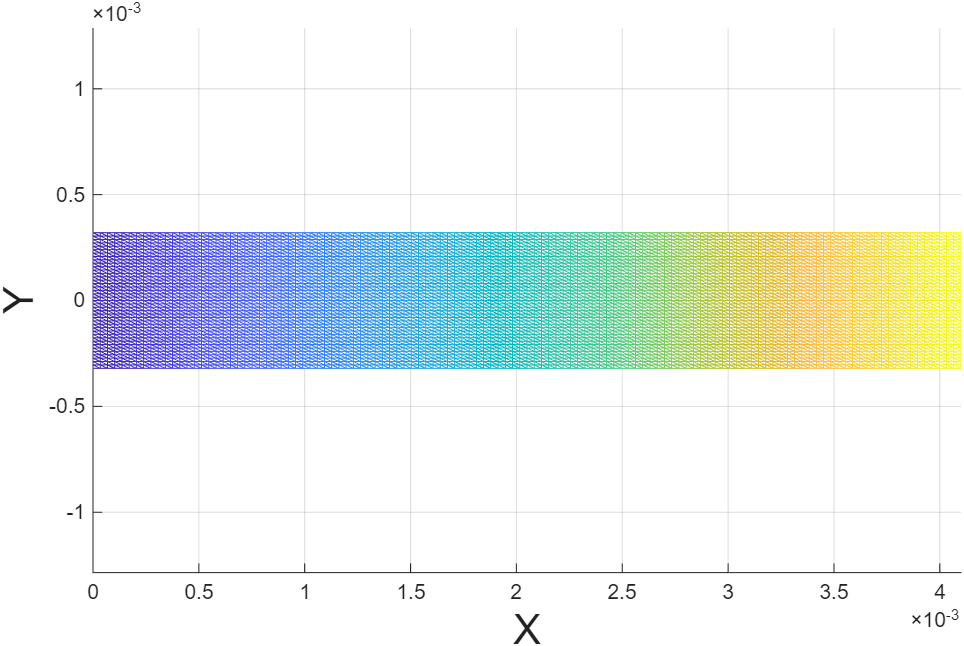
\includegraphics[width=0.8\textwidth]{part_1b_1}
    \caption{Numerical pressure profile for the 1D wedge bearing setup.}
    \label{fig:pressure_1d}
\end{figure}

\begin{figure}[H]
    \centering
    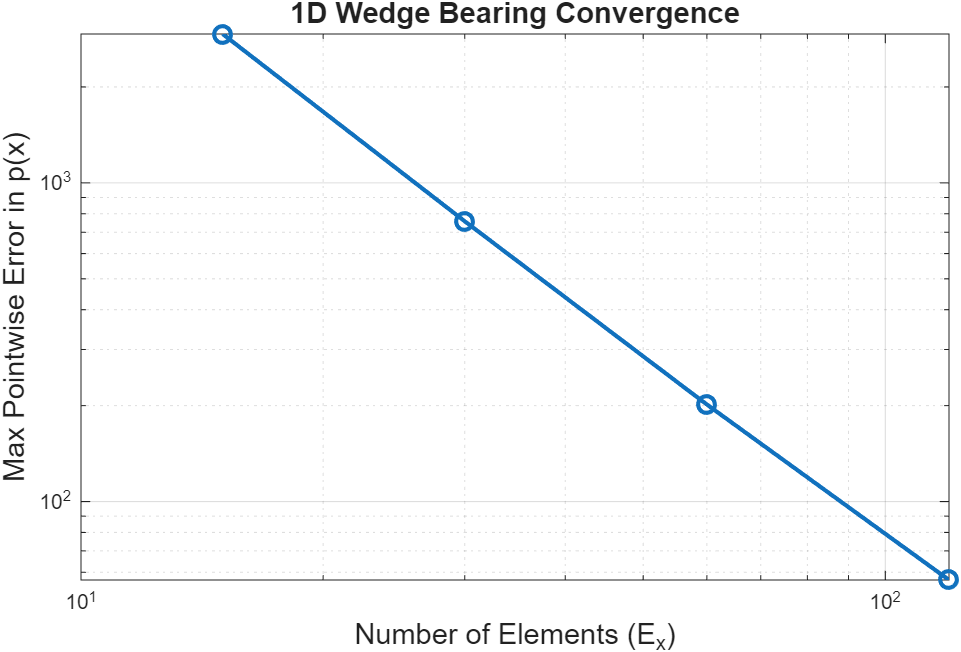
\includegraphics[width=0.8\textwidth]{part_1b_2}
    \caption{Log-log plot of the maximum pointwise error versus the number of elements ($E_x$), demonstrating near second-order convergence with a slope of $-1.90$.}
    \label{fig:convergence}
\end{figure}

\end{solution}



% -------------------------------------------------------
\begin{problem}{2(a)}

\end{problem}

\begin{solution}

In this section, we account for the compressibility of air as peak pressures rise significantly above ambient conditions. Under the isothermal assumption, the fluid density is proportional to the absolute pressure $p_a = p + p_{atm}$. The resulting compressible Reynolds equation is nonlinear:

\begin{equation}
    -\nabla \cdot \left( \frac{p_a h^3}{12\mu} \nabla p \right) + \frac{1}{2} \nabla \cdot (uhp) = -\frac{p_{atm}}{2} \nabla \cdot (uh)
\end{equation}

where $p$ is the relative pressure and $p=0$ on the boundary $\partial \Omega$.

\subsection*{Iterative Solution Methodology}
The nonlinearity in the stiffness matrix $\bar{A}(p_a)$ was treated using a successive iteration strategy. Starting with an initial guess of $p_a = p_{atm}$, the system was iterated using:
\begin{equation}
    R(\bar{A}(p_a) - \bar{C})R^T \underline{p} = R\bar{C}\underline{\bar{p}}_{atm}
\end{equation}
The solution reached convergence (maximum pressure change $< 10^{-3}$) in 13 iterations.

\subsection*{Results}
The following parameters and computed values characterize the compressible taper-flat configuration:

\begin{itemize}
    \item \textbf{Trailing height ($h_2$):} $2.500 \times 10^{-7}$ m
    \item \textbf{Pitch ($\gamma$):} $2.927 \times 10^{-5}$ radians
    \item \textbf{Computed Load ($F$):} $0.27828$ N
    \item \textbf{Center of Pressure ($x_p$):} $2.194 \times 10^{-3}$ m
\end{itemize}

\subsection*{Pressure Distribution}
The relative pressure distribution for the compressible case is shown in Figure \ref{fig:part_2a}. 

\begin{figure}[H]
    \centering
    
\includegraphics[width=0.8\textwidth]{part_2a}
    \caption{Pressure distribution for the compressible taper-flat slider configuration.}
    \label{fig:part_2a}
\end{figure}
\end{solution}

% -------------------------------------------------------
\begin{problem}{2(b)}

\end{problem}

\begin{solution}

Figure \ref{fig:comparison} presents a side-by-side comparison of the normalized pressure distributions for the three configurations analyzed in this study: the 2D incompressible taper-flat slider (Case 1a), the 1D incompressible pure wedge (Case 1b), and the 2D compressible taper-flat slider (Case 2a).

\subsection*{Analysis of Pressure Ranges and Distributions}
While all three subplots in Figure \ref{fig:comparison} are visually normalized by their respective maximum pressures ($p_{max}$) to clearly illustrate their profile shapes, their physical magnitudes differ significantly due to the underlying physics and boundary conditions:

\begin{itemize}
    \item \textbf{Case 1a (Incompressible 2D Taper-Flat):} The peak pressure is relatively low. The 2D nature of the domain allows fluid to ``leak'' out of the side edges ($y$-direction), relieving pressure. Furthermore, the $1^\circ$ leading taper delays the aggressive narrowing of the gap, limiting the pressure buildup at the entrance.
    \item \textbf{Case 1b (Incompressible 1D Wedge):} The maximum pressure is substantially higher than the 2D cases. This is primarily because the Neumann boundary conditions enforce strictly 1D flow, completely preventing any side leakage. Additionally, the removal of the leading taper means the geometric wedge acts over the full length of the slider, squeezing the fluid much more intensely from the very beginning.
    \item \textbf{Case 2a (Compressible 2D Taper-Flat):} The peak pressure is higher than its incompressible 2D equivalent (Case 1a). As the fluid is subjected to high pressures, its density increases, causing the fluid to effectively ``stiffen.'' This compressibility effect also alters the shape of the distribution slightly, shifting the peak pressure further toward the leading edge compared to the incompressible case.
\end{itemize}

\begin{figure}[H]
    \centering
    
\includegraphics[width=\textwidth]{part_2b}
    \caption{Side-by-side comparison of the pressure distributions for Cases 1a, 1b, and 2a. Note the difference in maximum pressure ($p_{max}$) magnitudes, particularly the increase in the 1D case.}
    \label{fig:comparison}
\end{figure}


\end{solution}


% -------------------------------------------------------
\begin{problem}{2(c)}

\end{problem}

\begin{solution}
Table \ref{tab:final_results} summarizes the computed load ($F$) and the normalized center of pressure ($x_p/L$) for the three slider configurations modeled in this assignment.

\begin{table}[H]
    \centering
    \renewcommand{\arraystretch}{1.3}
    \begin{tabular}{lcc}
        \toprule
        \textbf{Configuration Case} & \textbf{Load $F$ (N)} & \textbf{Center of Pressure $x_p/L$} \\
        \midrule
        \textbf{1a:} Incompressible 2D Taper-Flat & $0.2067$ & $0.5387$ \\
        \textbf{1b:} Incompressible 1D Pure Wedge & $8.1541$ & $0.5391$ \\
        \textbf{2a:} Compressible 2D Taper-Flat   & $0.2783$ & $0.5352$ \\
        \bottomrule
    \end{tabular}
    \caption{Comparison of the lifting load and normalized center of pressure across different fluid and geometric assumptions.}
    \label{tab:final_results}
\end{table}

\subsection*{Discussion of Findings}
Based on the results in Table \ref{tab:final_results}, several key physical insights can be drawn regarding the modeling of air bearings:

\begin{itemize}
    \item \textbf{The Impact of Side Leakage (1D vs. 2D):} 
    The 1D wedge model (Case 1b) predicts a load of $8.1541$ N, which is nearly 40 times larger than the realistic 2D model (Case 1a). By artificially restricting the flow to a single dimension (Neumann boundaries), the fluid cannot escape laterally. This creates an intense, artificial pressure ridge, grossly overestimating the slider's load-carrying capacity. This demonstrates why 2D modeling is strictly necessary for finite-width sliders.
    
    \item \textbf{The Effect of Compressibility (Case 1a vs. Case 2a):} 
    Introducing the compressible Reynolds equation (Case 2a) results in a load of $0.2783$ N, an increase of approximately 34\% over the incompressible baseline (Case 1a). As the air is squeezed into the narrow trailing gap, its absolute pressure rises, which proportionally increases the fluid density. This localized densification ``stiffens'' the air film, allowing it to generate more lift under the exact same geometric and kinematic conditions.
    
    \item \textbf{Stability of the Center of Pressure:} 
    Despite the massive variations in predicted load magnitudes, the normalized center of pressure ($x_p/L$) remains highly stable across all three models, situated at approximately $53.5\%$ to $53.9\%$ of the slider's length. The force consistently acts slightly downstream of the geometric center, which is characteristic of the wedge-like geometry squeezing fluid toward the trailing edge. 

    \item \textbf{Relative vs. Absolute Pressure:}
    In this case the atmospheric pressure acts on the exterior top of the slider \textbf{and} the bearing surface causing $p_{atm}$ to cancel.
    Using absolute pressure would result in an overestimated load equivalent to integrating $p_{atm}$ over the entire slider area.
    This would result in an order 1 error. 

\end{itemize}
\end{solution}

\end{document}